\documentclass[tikz,border=2pt]{standalone}
\usepackage{ctex}
\usetikzlibrary{calc}
\begin{document}
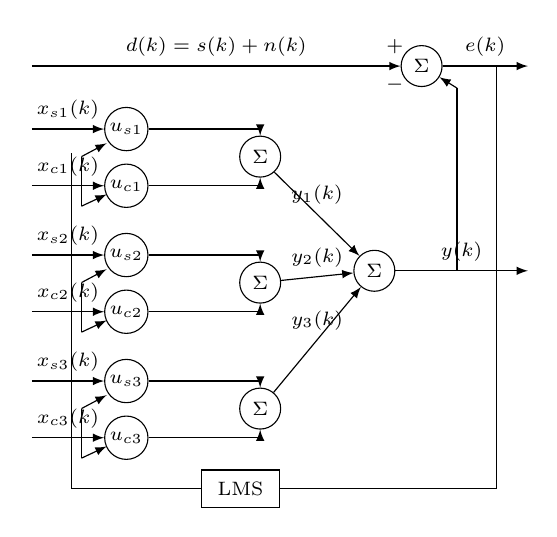
\begin{tikzpicture}[
  >=latex,
  font=\scriptsize,
  line/.style={draw, -latex, line width=0.42pt},
  plain/.style={draw, line width=0.42pt},
  sum/.style={draw, circle, minimum size=0.52cm, inner sep=0pt},
  gain/.style={draw, circle, minimum size=0.55cm, inner sep=0pt},
  block/.style={draw, rectangle, minimum width=1.0cm, minimum height=0.48cm, align=center}
]
\node[sum] (sume) at (5.2,5.55) {$\Sigma$};
\node[sum] (sumall) at (4.6,2.95) {$\Sigma$};
\node[block] (lms) at (2.9,0.18) {LMS};

\foreach \i/\y in {1/4.75,2/3.15,3/1.55} {
  \node[gain] (us\i) at (1.45,\y) {$u_{s\i}$};
  \node[gain] (uc\i) at (1.45,\y-0.72) {$u_{c\i}$};
  \node[sum] (sum\i) at (3.15,\y-0.35) {$\Sigma$};
  \draw[line] (0.25,\y) -- node[above] {$x_{s\i}(k)$} (us\i);
  \draw[line] (0.25,\y-0.72) -- node[above] {$x_{c\i}(k)$} (uc\i);
  \draw[line] (us\i) -| (sum\i);
  \draw[line] (uc\i) -| (sum\i);
  \draw[line] (sum\i) -- node[above] {$y_{\i}(k)$} (sumall);
  \draw[plain] (0.88,\y-0.98) -- (0.88,\y-0.35);
  \draw[line] (0.88,\y-0.35) -- (1.20,\y-0.18);
  \draw[line] (0.88,\y-0.98) -- (1.20,\y-0.83);
}

\draw[line] (0.25,5.55) -- node[above] {$d(k)=s(k)+n(k)$} (sume);
\draw[line] (sumall) -- node[above] {$y(k)$} (6.55,2.95);
\draw[plain] (5.65,2.95) -- (5.65,5.27);
\draw[line] (5.65,5.27) -- (sume);
\node at (4.86,5.80) {$+$};
\node at (4.86,5.32) {$-$};
\draw[line] (sume) -- node[above] {$e(k)$} (6.55,5.55);

\draw[plain] (6.15,5.55) -- (6.15,0.18) -- (3.40,0.18);
\draw[plain] (2.40,0.18) -- (0.75,0.18) -- (0.75,4.45);
\end{tikzpicture}
\end{document}
